\ifthenelse{\boolean{SUMMIT}}{
\begin{frame}
	\begin{center}
	\huge{Approach}
	\end{center}
\end{frame}
}{}

%\begin{frame}
%\frametitle{Goal of the project}
%%\begin{large}
%\textbf{Increasing the capturing performance in FreeBSD}\newline
%\begin{itemize}
%	\item<1-> Design and implementation of the new capturing software to
%		minimize the \textbf{CPU usage} and \textbf{packet loss} during sniffing.
%		\ifthenelse{\boolean{SUMMIT}}{
%		\begin{itemize}
%			\item<2-> The new implemented software should be transparent to the user-space applications
%		\end{itemize}
%		}{}
%\end{itemize}
%	
%\ifthenelse{\boolean{SUMMIT}}{}{
%\textbf{Supported Hardware:}
%\begin{itemize}
%	\item The following \emph{Intel GbE Controllers:}
%		\begin{itemize}
%			\item \small{\emph{8254x, 8257x, 8259x}}
%		\end{itemize}
%\end{itemize}
%}
%\end{frame}


\begin{frame}
\frametitle{Approach}
\begin{itemize}
	\item<1-> Using \textbf{ring} buffers
		\begin{itemize}
			\item<1-> for eliminating the memory allocations
				\ifthenelse{\boolean{SUMMIT}}{
				\begin{itemize}
					\item<1-> reusing packet buffers: no new allocations\newline
				\end{itemize}
				}{}
		\end{itemize}

	\item<2-> Using shared memory buffers (\emph{memory \textbf{mapping}})
		\begin{itemize}
			\item<2-> Eliminating the packet copy operations				
				\ifthenelse{\boolean{SUMMIT}}{
				\begin{itemize}
					\item<2-> mapping DMA buffers into the user-space\newline
				\end{itemize}
				}{}
		\end{itemize}
%	\item<4-> Modifying \emph{libpcap}
%		\begin{itemize}
%			\item<4-> libpcap-apps don't require modifications\newline
%		\end{itemize}
	\item<3->[$\Rightarrow$] Project Name: $ring + mapping = \textbf{ringmap}$
\end{itemize}
\end{frame}


\begin{frame}
\frametitle{Approach 2}
\textbf{Supported Hardware:}
\begin{itemize}
	\item The following \emph{Intel GbE Controllers:}
		\begin{itemize}
			\item \small{\emph{8254x, 8257x, 8259x}}\newline
		\end{itemize}
\end{itemize}

\textbf{Modified \emph{libpcap}}
\begin{itemize}
	\item Libpcap is adapted to \emph{ringmap}
	\begin{itemize}
		\item libpcap-apps don't require modifications
			\begin{itemize}
				\item tcpdump, wireshark, etc\ldots
			\end{itemize}
	\end{itemize}
\end{itemize}
\end{frame}

\begin{frame}
\frametitle{Overview}
\begin{center}
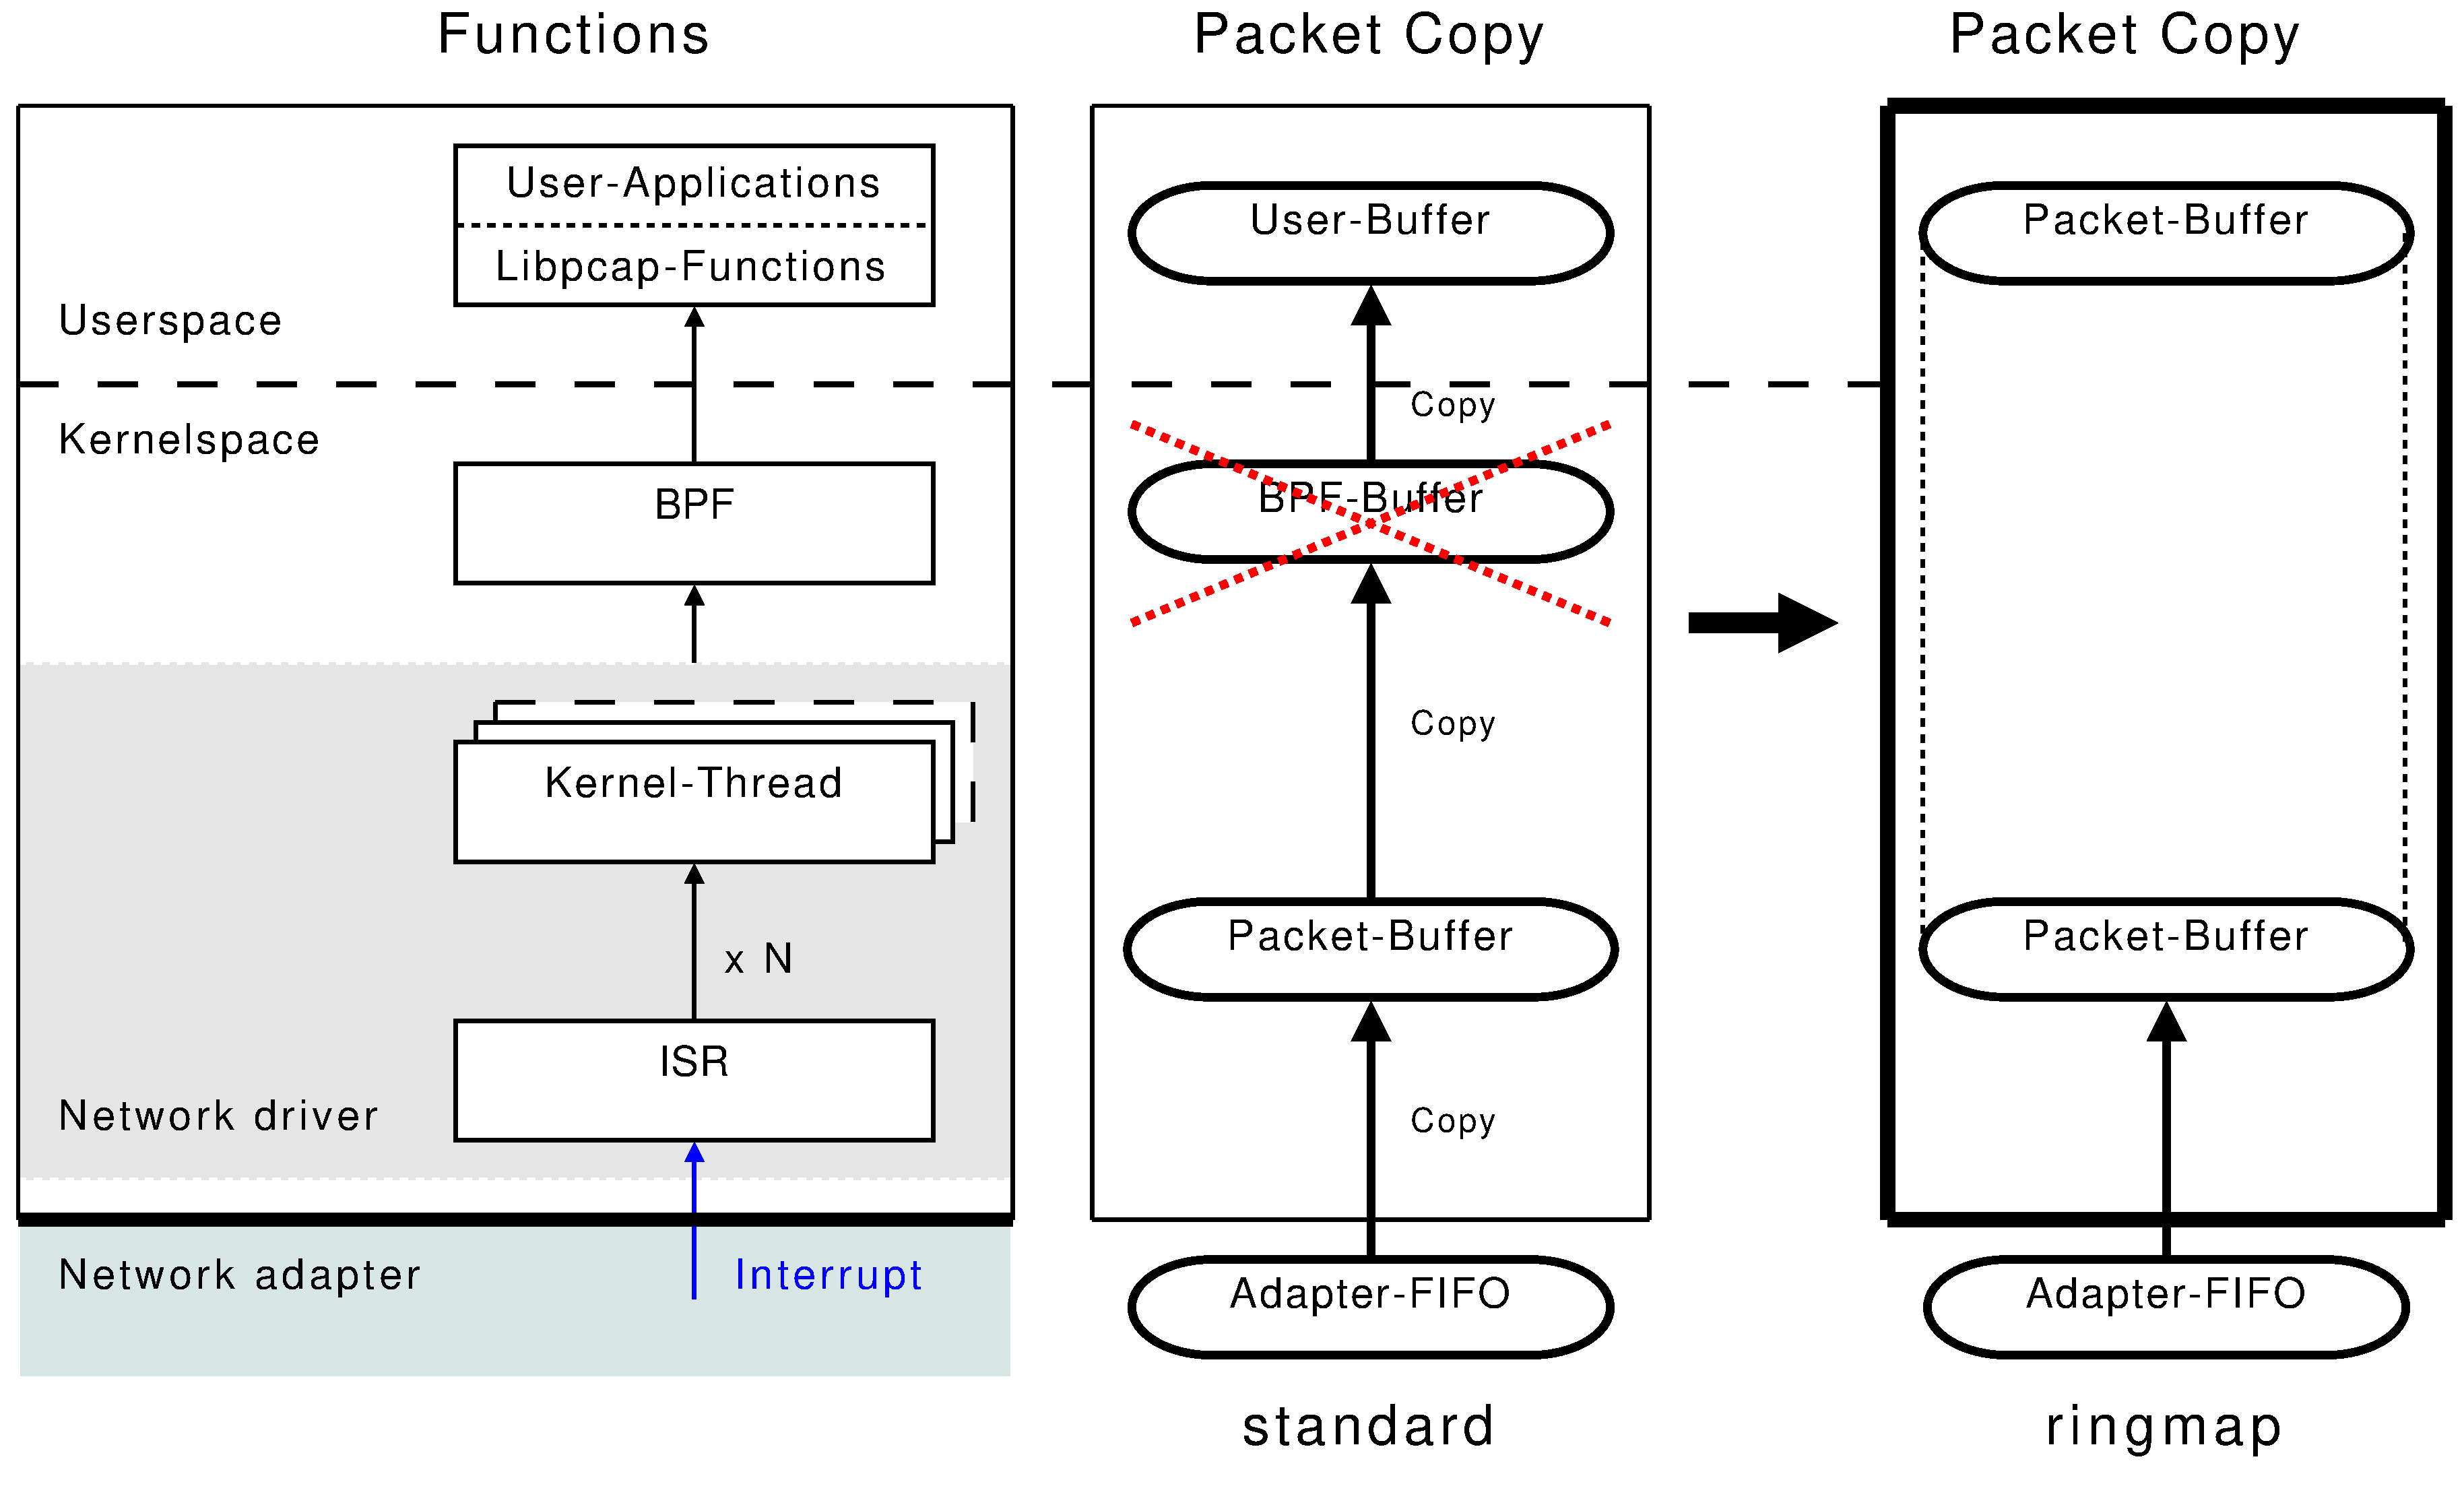
\includegraphics [height=55mm,width=100mm]{pics/Ueberblick_new_summit}
\end{center}
\end{frame}

